\documentclass[conference]{IEEEtran}
\IEEEoverridecommandlockouts
% The preceding line is only needed to identify funding in the first footnote. If that is unneeded, please comment it out.
\usepackage{cite}
\usepackage{amsmath,amssymb,amsfonts}
\usepackage{algorithmic}
\usepackage{graphicx}
\usepackage{textcomp}
\usepackage{xcolor}
\usepackage{hyperref}
\def\BibTeX{{\rm B\kern-.05em{\sc i\kern-.025em b}\kern-.08em
    T\kern-.1667em\lower.7ex\hbox{E}\kern-.125emX}}
\begin{document}

\title{HASHIRU: Hierarchical Agent System for Hybrid Intelligent Resource Utilization}

\author{\IEEEauthorblockN{Kunal Pai}
\IEEEauthorblockA{\textit{UC Davis} \\
kunpai@ucdavis.edu}
\and
\IEEEauthorblockN{Parth Shah}
\IEEEauthorblockA{\textit{Independent Researcher} \\
helloparthshah@gmail.com}
\and
\IEEEauthorblockN{Harshil Patel}
\IEEEauthorblockA{\textit{UC Davis} \\
hpppatel@ucdavis.edu}
\and
\IEEEauthorblockN{Saisha Shetty}
\IEEEauthorblockA{\textit{UC Davis} \\
spshetty@ucdavis.edu}
}

\maketitle

\section{Introduction}\label{sec:introduction}

The landscape of Artificial Intelligence (AI) is being reshaped by the rapid advancements in Large Language Models (LLMs), which exhibit profound capabilities in language understanding, generation, reasoning, and planning \cite{brown2020language, devlin2019bert, raffel2020exploring}. This progress has catalyzed the development of sophisticated AI agents capable of autonomous task execution. Increasingly, the focus is shifting from single-agent systems to Multi-Agent Systems (MAS), where collaborative teams of specialized agents address complex problems beyond the scope of individual agents \cite{dorri2018multi, wooldridge2009introduction}. Such collaborative approaches hold significant potential in diverse domains like scientific discovery \cite{boiko2023emergent}, software engineering \cite{qian2023communicative}, data analysis, and strategic decision-making \cite{wang2023decision}. The growing complexity of tasks, highlighted by benchmarks demanding advanced mathematical reasoning (e.g., GSM8K \cite{cobbe2021gsm8k}, SVAMP \cite{patel2021svamp}), coding (e.g., HumanEval \cite{chen2021codex}, CoDocBench \cite{pai2024codocbench}), and graduate-level technical knowledge and reasoning \cite{phan2025humanitysexam}, further underscores the need for agentic systems capable of effectively coordinating diverse cognitive resources \cite{wen2024benchmarkingcomplexinstructionfollowingmultiple}.

Despite this promise, contemporary agentic frameworks often encounter significant limitations. Many suffer from \textbf{rigidity}, relying on predefined agent roles and static team structures that hinder adaptation to dynamic task requirements \cite{zhang2023building}. Furthermore, \textbf{resource obliviousness} is prevalent; systems frequently lack mechanisms to monitor and optimize computational resources like API costs, memory usage, and CPU load, leading to inefficiency, particularly when scaling or deploying in resource-constrained environments \cite{park2023generative}. This is often exacerbated by a reliance on powerful, proprietary cloud-based LLMs, incurring substantial operational expenses. \textbf{Model homogeneity}, the default use of a single powerful LLM for all sub-tasks, neglects the potential efficiency gains from employing a diverse ecosystem of models, including smaller, specialized, or locally-run alternatives \cite{zhou2023agents}. Lastly, while \textbf{tool use} is fundamental \cite{yao2022react, parisi2022talm}, the ability for agents to autonomously \textbf{create and integrate new tools} during operation remains limited, restricting dynamic functional extension and long-term self-improvement without human intervention \cite{wang2023voyager}.

To address these challenges, we introduce \textbf{HASHIRU (Hierarchical Agent System for Hybrid Intelligent Resource Utilization)}, a novel MAS framework designed for enhanced flexibility, resource efficiency, and adaptability. HASHIRU employs a hierarchical structure led by a central ``CEO'' agent that dynamically manages a team of specialized ``employee'' agents, instantiated on demand for specific sub-tasks. A core tenet of HASHIRU is its \textbf{hybrid intelligence} approach, strategically prioritizing smaller (e.g., 3B--7B parameter), locally-run LLMs, often accessed via frameworks like Ollama \cite{ollama}, to promote cost-effectiveness and computational efficiency. While prioritizing local resources, the system retains the flexibility to integrate external APIs and potentially more powerful models when justified by task complexity and resource availability, under the CEO's management.

The primary contributions of this work are:
\begin{enumerate}
    \item A novel MAS architecture combining a \textbf{hierarchical control structure} with \textbf{dynamic, resource-aware agent lifecycle management} (hiring/firing). This management is explicitly governed by computational budget constraints (cost, memory usage, concurrency) and incorporates an economic model with hiring/firing costs to discourage excessive churn.
    \item A \textbf{hybrid intelligence model} that prioritizes cost-effective, local LLMs while adaptively incorporating external APIs and potentially larger models, optimizing the efficiency-capability trade-off.
    \item An integrated mechanism enabling the \textbf{autonomous creation of API tools}, allowing the system to dynamically extend its functional repertoire in response to task demands.
    \item The application of an \textbf{economic model} (hiring/firing fees) to agent management, promoting efficient resource allocation and team stability.
\end{enumerate}

This paper details the design and rationale behind HASHIRU. Section \ref{sec:background} discusses related work in agent architectures, dynamic management, resource allocation, model heterogeneity, and tool use. Section 3 elaborates on the HASHIRU architecture and its core mechanisms. Section 4 presents experimental results (or outlines planned experiments), followed by discussion and conclusion in Sections 5 and 6.

\section{Background and Related Work} \label{sec:background}

The concept of intelligent agents has evolved significantly from early work in symbolic AI and distributed problem-solving \cite{russell2010artificial, shoham1994agent} to the current era dominated by LLMs. Modern agentic frameworks leverage LLMs as their cognitive core, enabling sophisticated reasoning, planning, and interaction capabilities \cite{wang2023survey, xi2023rise}. HASHIRU builds upon this foundation while addressing specific limitations observed in the current state-of-the-art.

\subsection{Agent Architectures: Hierarchy and Dynamics}
MAS architectures vary widely, including flat, federated, and hierarchical structures \cite{dorri2018multi, horling2004survey}. Hierarchical models offer clear control flow and efficient task decomposition but risk bottlenecks and rigidity \cite{gaston2005agenta,gaston2005agentb}. HASHIRU utilizes a \textbf{CEO-Employee hierarchy} for centralized coordination but distinguishes itself through \textbf{dynamic team composition}. Unlike systems with static hierarchies or predefined roles (e.g., CrewAI \cite{crewai}, ChatDev \cite{qian2023communicative}), HASHIRU's CEO actively manages the employee pool based on runtime needs and resource constraints.

\subsection{Dynamic Agent Lifecycle Management}
The ability of an MAS to adapt its composition dynamically is crucial for complex environments \cite{valckenaers2005trends}. Various triggers for agent creation or deletion have been explored, often tied to task structure or environmental changes. HASHIRU introduces a specific mechanism where the CEO agent makes \textbf{hiring and firing decisions} based on a cost-benefit analysis considering agent performance, operational costs (API fees, inferred compute), memory footprint (tracked explicitly as a percentage of available resources), and agent concurrency limits. Furthermore, HASHIRU incorporates an \textbf{economic model} with explicit ``starting bonus'' (hiring) and ``invocation'' (usage) costs. This introduces economic friction, aiming to prevent excessive agent initialization or usage for marginal gains and promote team stability, a nuance often missing in simpler dynamic composition strategies.

\subsection{Resource Management and Agent Economies}
Resource awareness is critical for scalable and deployable MAS. Research areas in economics explore mechanisms like market-based auctions or contract nets for resource allocation \cite{clearwater1996market}. HASHIRU implements a more \textbf{centralized, budget-constrained resource management model}. The CEO operates within defined limits for financial cost, memory usage (as a percentage of total available memory), and concurrent agent count. This direct management, particularly the focus on memory percentage, suggests an orientation towards practical deployment, potentially on local hardware or edge devices with finite resources, contrasting with cloud-centric systems assuming elastic resources \cite{park2023generative}. Frameworks like AutoGen \cite{wu2023autogen} and LangGraph \cite{langgraph} typically rely on implicit cost tracking via API keys without such explicit multi-dimensional resource budgeting and control.

\subsection{Hybrid Intelligence and Heterogeneous Models}
Leveraging diverse LLMs with varying capabilities, costs, and latencies is an emerging trend \cite{zhou2023agents}. Techniques like model routing aim to select the optimal model for specific sub-tasks. HASHIRU embraces \textbf{model heterogeneity} with a specific strategic focus: \textbf{prioritizing smaller (3B--7B), locally-run models via Ollama integration} \cite{ollama}. This emphasizes cost-efficiency, low latency for simpler tasks, and potential privacy advantages over systems defaulting to large, proprietary cloud APIs (e.g., GPT-4 \cite{openai2023gpt4}, Claude 3 \cite{anthropic2024claude}). While capable of integrating external APIs (potentially invoking larger models), HASHIRU's default operational stance represents a distinct balance point in the capability vs. efficiency trade-off.

\subsection{Tool Use and Autonomous Tool Creation}
The ability to use external tools (APIs, functions, databases) is a cornerstone of modern agents, enabled by frameworks like ReAct \cite{yao2022react} and built-in function calling \cite{openai_func_calling}. Most systems rely on a predefined tool suite. HASHIRU advances this by incorporating a mechanism for \textbf{autonomous API tool creation}. When a required functionality is missing, the CEO can commission the generation (potentially via a specialized agent or code generation process) and deployment of a new API tool within the HASHIRU ecosystem. This capability for self-extension differentiates HASHIRU from systems limited to static toolsets and moves towards greater operational autonomy and adaptability \cite{wang2023voyager, park2023generative}.

In summary, HASHIRU integrates concepts from hierarchical control, dynamic MAS, resource management, and tool use, but its novelty lies in the synergistic combination of: (1) dynamic, resource-aware hierarchical management with (2) an economic model for stability, (3) a local-first hybrid intelligence strategy, and (4) integrated autonomous tool creation capabilities. This combination targets key limitations in current agentic systems concerning efficiency, adaptability, cost, and autonomy.

\section{HASHIRU System Architecture}
\label{sec:architecture}

The architecture of HASHIRU is designed to directly address the challenges of rigidity, resource obliviousness, and limited adaptability outlined in Section~\ref{sec:introduction}. It implements a hierarchical, dynamically managed multi-agent system optimized for hybrid resource utilization. This section details the core components and mechanisms underpinning HASHIRU's operation.

\subsection{Overview}
HASHIRU operates on a hierarchical model conceptually similar to a business organization, featuring a central coordinating agent (``CEO'') and specialized task-executing agents (``Employees''). Key architectural tenets include:
\begin{itemize}
    \item \textbf{Centralized Coordination within a Dynamic Hierarchy:} A CEO agent manages overall strategy, task allocation, and team composition.
    \item \textbf{Dynamic Lifecycle Management:} Employee agents are instantiated (hired) and terminated (fired) based on runtime requirements and resource constraints, governed by an economic model.
    \item \textbf{Hybrid Intelligence:} Strategic preference for local, computationally cheaper LLMs, while retaining access to external APIs and potentially more powerful models.
    \item \textbf{Explicit Resource Management:} Continuous monitoring and control of costs, memory usage, and agent concurrency against defined budgets.
    \item \textbf{Adaptive Tooling:} Utilization of predefined tools alongside the capability for autonomous creation of new API tools.
\end{itemize}
Figure \ref{fig:arch} illustrates the overall structure and interaction flow.

\begin{figure}[ht]
    \centering
    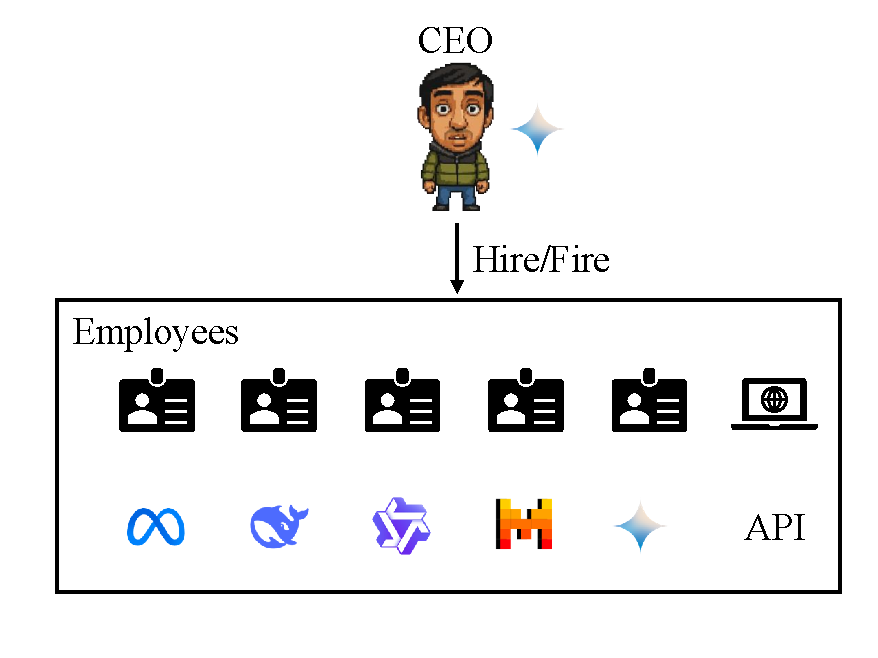
\includegraphics[width=0.45\textwidth]{HASHIRU.pdf}
    \caption{High-level architecture of the HASHIRU system, illustrating the CEO-Employee hierarchy.}
    \label{fig:arch}
\end{figure}

\subsection{Hierarchical Structure: CEO and Employee Agents}
The system employs a two-tiered hierarchy:

\begin{itemize}
    \item \textbf{CEO Agent:} This singleton agent serves as the central coordinator and entry point. Its primary responsibilities include:
        \begin{itemize}
            \item Receiving and interpreting the primary user query or task.
            \item Decomposing the main task into smaller, manageable sub-tasks.
            \item Identifying the capabilities required for each sub-task.
            \item Managing the pool of Employee agents (see Section \ref{subsec:dynamic_mgmt}).
            \item Assigning sub-tasks to suitable, active Employee agents.
            \item Monitoring the progress and performance of Employee agents.
            \item Synthesizing the results from Employee agents into a coherent final output or response.
            \item Managing the system's overall resource budget (see Section \ref{subsec:resource_mgmt}).
            \item Initiating the creation of new tools when required (see Section \ref{subsec:tooling}).
        \end{itemize}
    \item \textbf{Employee Agents:} These are specialized agents instantiated by the CEO to perform specific sub-tasks. Each Employee agent typically wraps an LLM (local via Ollama \cite{ollama} or external via API) or provides access to a specific tool/API. Key characteristics include:
        \begin{itemize}
            \item Specialization: Possessing capabilities tailored to certain types of sub-tasks (e.g., code generation, data analysis, information retrieval).
            \item Dynamic Existence: Created and destroyed by the CEO based on need and performance.
            \item Task Execution: Receives a sub-task description and context from the CEO, executes it, and returns the result.
            \item Resource Consumption: Associated with specific resource costs (e.g., API call costs, memory footprint) tracked by the system.
        \end{itemize}
\end{itemize}
This hierarchical structure facilitates organized task decomposition and result aggregation under centralized control, while the dynamic nature of the Employee pool provides flexibility.

\subsection{Dynamic Agent Lifecycle Management}
\label{subsec:dynamic_mgmt}
A core innovation in HASHIRU is the CEO's ability to dynamically manage the Employee agent team through ``hiring'' (instantiation) and ``firing'' (termination). This process is driven by a cost-benefit analysis aimed at optimizing task performance within resource constraints.

When a new sub-task requires capabilities not readily available or efficiently provided by the current pool of active Employee agents, the CEO may decide to hire a new agent. Conversely, if an agent is underperforming, consistently idle, excessively costly, or if resource limits are approached, the CEO may decide to fire it. This decision considers multiple factors:
\begin{itemize}
    \item \textbf{Task Requirements:} The specific capabilities needed for pending sub-tasks.
    \item \textbf{Agent Performance Metrics:} Historical success rate, quality of output, or efficiency of existing agents relevant to the task type.
    \item \textbf{Operational Costs:} API costs, estimated computational load, or other costs associated with using the agent's underlying model or tools.
    \item \textbf{Memory Footprint:} The amount of system memory the agent consumes, tracked as a percentage of the total available memory allocated to HASHIRU.
    \item \textbf{Agent Concurrency:} The current number of active Employee agents relative to a predefined limit.
\end{itemize}

Crucially, HASHIRU incorporates an \textbf{economic model} for agent lifecycle events:
\begin{itemize}
    \item \textbf{Hiring Cost (``Starting Bonus''):} A one-time cost incurred when a new agent is instantiated, representing setup overhead.
    \item \textbf{Invocation Cost (``Salary''):} A multi-time cost incurred when an agent is used, representing load on the system, or on payment methods, for using an agent.
\end{itemize}
These explicit transaction costs discourage excessive agent churn, promoting stability. The CEO must evaluate if the anticipated long-term benefit of replacing an agent outweighs the immediate hiring and firing costs plus any difference in ongoing operational costs. This mechanism directly combats system rigidity and allows adaptation while actively managing computational budgets and preventing wasteful high-frequency agent turnover.

\subsection{Hybrid Intelligence and Model Management}
HASHIRU is designed for \textbf{hybrid intelligence}, leveraging a diverse set of cognitive resources. It strategically prioritizes the use of smaller (e.g., 3B--7B parameter), cost-effective LLMs that can be run locally via frameworks like Ollama \cite{ollama}. This approach enhances efficiency, reduces reliance on expensive external APIs, and potentially improves privacy and latency for certain tasks.

However, the system is not restricted to local models. The CEO agent can integrate and utilize:
\begin{itemize}
    \item \textbf{External LLM APIs:} Access to powerful proprietary models (e.g., GPT-4 \cite{openai2023gpt4}, Claude 3 \cite{anthropic2024claude}) when deemed necessary for complex reasoning or specialized knowledge, subject to cost-benefit analysis.
    \item \textbf{External Tool APIs:} Integration with third-party software or data sources.
    \item \textbf{Self-Created APIs:} Tools generated by HASHIRU itself (see Section \ref{subsec:tooling}).
\end{itemize}
The CEO manages this heterogeneous pool, selecting the most appropriate resource (local model, external API, tool) for a given sub-task based on perceived difficulty, required capabilities, and the current resource budget status. This allows HASHIRU to balance cost-effectiveness and computational efficiency with the need for high capability when required.

\subsection{Resource Monitoring and Control}
\label{subsec:resource_mgmt}
Explicit resource management is central to HASHIRU's design, moving beyond simple API key cost tracking. The system, coordinated by the CEO, actively monitors:
\begin{itemize}
    \item \textbf{Financial Costs:} Accumulating costs from external API calls.
    \item \textbf{Memory Usage:} Tracking the memory footprint of active Employee agents, specifically as a percentage of a predefined total available memory resource.
    \item \textbf{Agent Concurrency:} Maintaining a count of concurrently active Employee agents.
\end{itemize}
These metrics are monitored against predefined \textbf{budget limits} or hard caps. If initiating an action (like hiring a new agent) would exceed a budget limit (e.g., push memory usage over 90\% of allocated, or exceed the maximum concurrent agent count), the action is prevented. This mechanism ensures the system operates within defined operational constraints, crucial for deployment on devices with limited resources or under strict financial budgets.

\subsection{Tool Utilization and Autonomous Creation}
\label{subsec:tooling}
Like many modern agent systems, HASHIRU's agents can utilize predefined tools (functions, external APIs, databases) to interact with the environment and perform actions beyond pure text generation \cite{yao2022react, openai_func_calling}.

A distinctive feature of HASHIRU is its capability for \textbf{integrated, autonomous tool creation}. If the CEO agent determines, through task analysis or failure analysis of existing agents, that a specific functional capability is required but not available through existing Employee agents or tools, it can initiate a process to create a new tool. This typically involves:
\begin{enumerate}
    \item Defining the specification for the required tool (inputs, outputs, functionality).
    \item Commissioning the generation of the necessary logic (e.g., code implementing the functionality, potentially involving API calls to external services using provided credentials, possibly generated by a specialized code-generating Employee agent).
    \item Deploying this logic as a new, callable API endpoint accessible within the HASHIRU ecosystem.
    \item Potentially instantiating a new Employee agent dedicated to utilizing this newly created tool.
\end{enumerate}
This mechanism allows HASHIRU to dynamically extend its own functional repertoire over time, tailoring its capabilities to the tasks it encounters without requiring direct manual intervention for every new function, thereby enabling greater autonomy and long-term adaptation.


\section{Experimental Setup}
\label{sec:experiments}

To evaluate the performance, efficiency, and adaptability of HASHIRU, we designed a set of experiments targeting its core architectural features. Our evaluation focuses on assessing the benefits of dynamic resource-aware management, the hybrid intelligence model, and the autonomous tool creation capability compared to relevant baselines. Specifically, we investigate:
\begin{itemize}
    \item The impact of dynamic agent management with economic constraints on resource utilization (cost, memory) and task performance compared to static configurations.
    \item The effectiveness of the hybrid (local-first) model strategy versus homogeneous (cloud-only or local-only) approaches across tasks of varying complexity.
    \item The system's ability to autonomously create and utilize necessary tools when faced with novel functional requirements within a task.
\end{itemize}

\subsection{Evaluation Tasks}
\label{subsec:tasks}
We selected tasks demanding complex reasoning, multi-perspective analysis, and interaction, suitable for exercising HASHIRU's hierarchical coordination and dynamic capabilities. The tasks fall into two main categories:

\subsubsection{Academic Paper Review}
This task evaluates HASHIRU's capacity to critically assess academic work by simulating the peer-review process. Given one or more scientific papers (e.g., in PDF format), the system must generate a review summary and ultimately recommend acceptance or rejection. This probes HASHIRU's ability to decompose evaluation criteria, delegate tasks to specialized agents (e.g., novelty assessment, methodological rigor, clarity), and manage resources effectively across long and complex documents.

\subsubsection{Reasoning and Problem-Solving Tasks}
To evaluate broader reasoning, knowledge retrieval, and problem-solving capabilities under different constraints, we employ a set of challenging benchmarks and puzzle-like tasks:
\begin{itemize}
    \item \textbf{Humanity's Last Exam \cite{phan2025humanitysexam}:} A benchmark designed to test graduate-level technical knowledge and complex reasoning across multiple domains. Success requires deep understanding and sophisticated problem-solving, likely necessitating access to powerful external LLMs managed effectively within HASHIRU's hybrid framework.
    \item \textbf{NYT Connections:} This popular puzzle requires identifying hidden semantic relationships or themes to categorize 16 words into four distinct groups. Solving this involves associative reasoning, broad world knowledge, and potentially hypothesis testing across different potential groupings, testing knowledge access and combinatorial reasoning coordination.
    \item \textbf{Wordle:} The daily word puzzle requires deductive reasoning to identify a five-letter word within six guesses, using feedback on correct letters and positions. This tests logical deduction, constraint satisfaction, and vocabulary knowledge. It serves as a good test case for comparing the efficiency (speed, cost, number of guesses) of local versus external models for iterative reasoning. We assume interaction via a simulated game environment.
    \item \textbf{Globle:} This geographic deduction game requires identifying a target country based on proximity feedback from guesses. It tests geographic knowledge retrieval, spatial reasoning, and iterative strategy refinement based on feedback (distance, direction). We assume interaction via a simulated game environment. 
\end{itemize}
These diverse reasoning tasks challenge the system's ability to leverage appropriate cognitive resources (local vs. external models), potentially create simple tools, and coordinate problem-solving strategies effectively.

\subsection{Baselines for Comparison}
\label{subsec:baselines}
To quantify the benefits of HASHIRU's features, we will compare its performance against several baseline configurations:
\begin{itemize}
    \item \textbf{Static-HASHIRU:} A version with a fixed, predefined set of Employee agents (e.g., one generalist agent per potential role identified in paper analysis), disabling dynamic hiring/firing.
    \item \textbf{Cloud-Only HASHIRU:} HASHIRU operating exclusively with a powerful external LLM API and online function-calling for all agents, disabling the use of local models.
    \item \textbf{Local-Only HASHIRU:} HASHIRU operating exclusively with smaller, local LLMs (e.g., selected models via Ollama) for all agents.
    \item \textbf{HASHIRU (No-Economy):} HASHIRU with dynamic hiring/firing enabled but without the explicit costs, to isolate the impact of the economic model on agent churn and stability.
    % \item \textbf{[Optional] Other Frameworks:} If feasible, configure AutoGen \cite{wu2023autogen} or CrewAI \cite{crewai} with a similar hierarchical structure to solve a subset of the tasks for comparison.
\end{itemize}

\subsection{Evaluation Metrics}
\label{subsec:metrics}
We will evaluate performance using a combination of quantitative and qualitative metrics:
\begin{itemize}
    \item \textbf{Task Success Rate / Quality:}
        \begin{itemize}
            \item Percentage of tasks successfully completed (binary for games, potentially graded for analysis based on rubrics).
            \item Quality of output for analysis tasks (human evaluation based on relevance, coherence, accuracy, completeness).
            \item Accuracy for information extraction tasks.
            \item Number of guesses/turns required for game tasks.
        \end{itemize}
    \item \textbf{Resource Consumption:}
        \begin{itemize}
            \item Total cost incurred from external API calls.
            \item Peak and average memory usage (\% of allocated budget).
            \item Wall-clock time per task.
            \item Number and type (local/external) of LLM calls.
        \end{itemize}
    \item \textbf{System Dynamics and Adaptability:}
        \begin{itemize}
            \item Number of Employee agents hired and fired during tasks.
            \item Frequency of agent churn (hires+fires / task duration or steps).
            \item Number and utility of autonomously created tools (if applicable).
        \end{itemize}
\end{itemize}



\bibliography{references}
\bibliographystyle{plain}

\end{document}
